\documentclass[11pt]{article}

\usepackage[margin=1in]{geometry}
\usepackage[utf8]{inputenc}
\usepackage[T1]{fontenc}
\usepackage{amsmath,amssymb}
\usepackage{booktabs}
\usepackage{array}
\usepackage{graphicx}
\usepackage{xcolor}
\usepackage{enumitem}
\usepackage{caption}
\usepackage{longtable}
\usepackage{float}
\usepackage{algorithm}
\usepackage{algpseudocode}
\usepackage[hidelinks,colorlinks=false]{hyperref}
\usepackage[noabbrev,capitalise]{cleveref}

\setlength{\parindent}{0pt}
\setlength{\parskip}{6pt}
\emergencystretch=3em

\definecolor{cIndigo}{HTML}{3A4CC4}
\definecolor{cAmber}{HTML}{96590A}
\definecolor{cInk2}{HTML}{525A6C}
\definecolor{cPanel}{HTML}{F6F7F9}
\definecolor{cRule}{HTML}{BFC6D3}

\newcommand{\dgraph}{d_{\mathrm{graph}}}
\newcommand{\zv}{\mathbf{z}}

\title{\vspace{-2em}\textbf{Latent-Space Diagnostics}\\[0.3em]
\large Two-Room's encoder and predictor geometry: distances, dimensionality, and where
$\tau_{\mathrm{fwd}}$'s calibration bug actually comes from}
\author{Companion to \texttt{predictor-stitching.tex}}
\date{6 September 2026}

\begin{document}
\maketitle
\vspace{-1.5em}

\section{Purpose}

Before trusting any threshold built on top of the encoder or the predictor, it helps to look
directly at the geometry they produce. This document collects diagnostic figures on
Two-Room's 27{,}675-landmark B0 landmark set, generated by \texttt{scripts/latent\_diagnostics.py}.
It is a companion to \texttt{predictor-stitching.tex}, which develops the IDM-ensemble/predictor
verification mechanism these figures inform --- in particular \cref{fig:predictor-history} is
the direct source of the $\tau_{\mathrm{fwd}}$ mis-scaling diagnosed in that document's E2
section, and \cref{fig:idm-variance} is a visual confirmation of that document's finding that
ensemble variance does not discriminate real transitions from the wide candidate pool.

\begin{figure}[H]
\centering
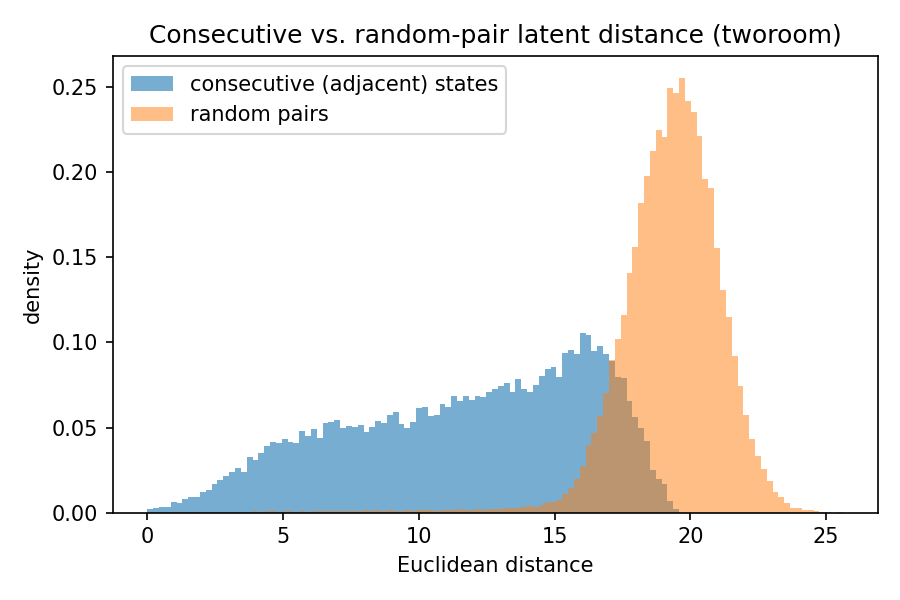
\includegraphics[width=0.75\linewidth]{figures/tworoom_adjacent_vs_random.png}
\caption{Consecutive (real, same-episode) states sit much closer together (mean $11.75$,
median $12.43$) than random pairs (mean $19.25$) --- the encoder clearly separates temporal
neighbors from arbitrary states, which is the entire precondition for a distance-based
identification-edge threshold to mean anything.}
\label{fig:adjacent-vs-random}
\end{figure}

\begin{figure}[H]
\centering
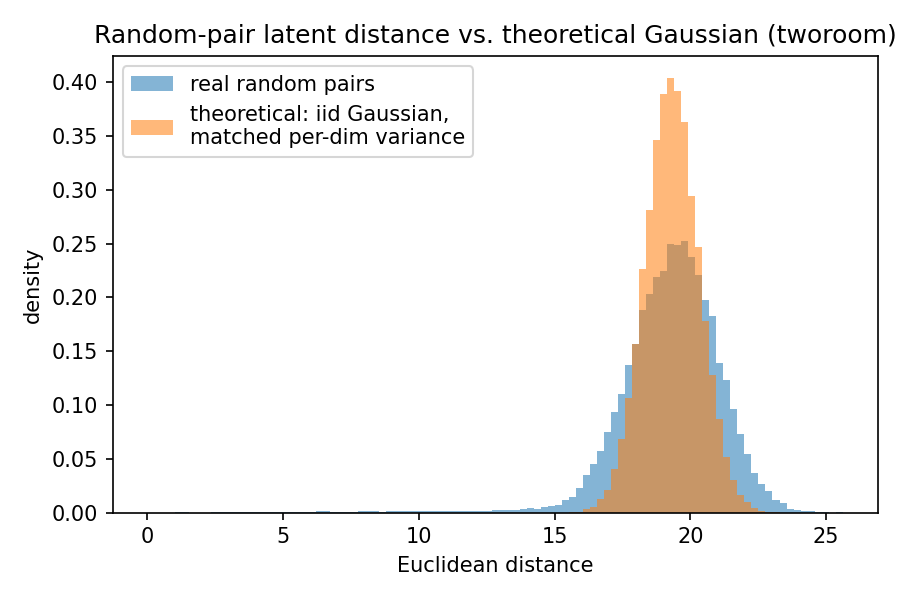
\includegraphics[width=0.75\linewidth]{figures/tworoom_random_vs_theoretical.png}
\caption{Real random-pair distances (mean $19.25$) closely track a theoretical reference ---
two independent Gaussian vectors with the same per-dimension variance as the real embedding,
sampled and measured the same way (mean $19.32$). At the level of pairwise distance
statistics, Two-Room's embedding looks close to an anisotropic Gaussian blob, not a
sharply-folded manifold --- a sanity check behind \texttt{main.tex}'s calibration formula,
which implicitly assumes something like this.}
\label{fig:random-vs-theoretical}
\end{figure}

\textbf{Correction (6 September 2026):} the two figures below were originally built by
feeding the predictor a single real action, zero-padded into the 10-dim slot
$\mathrm{action\_encoder}$ expects, and comparing its output one real step later. That
invocation was wrong. The checkpoint's actual training convention
(\texttt{docs/lewm.txt}, Appendix D) applies a \textbf{frame-skip of 5}: one predictor call
consumes the concatenation of \textbf{5 consecutive real actions} ($5\times2{=}10$ dims,
exactly matching $\mathrm{action\_encoder}$'s input size with no padding at all) and
predicts the state \textbf{5 real steps} later, not 1. Every figure below is now built the
corrected way; see \texttt{scripts/latent\_diagnostics.py}'s
\texttt{build\_block\_history\_chains}. The original padding-based numbers are kept in
memory (\texttt{[[lewm-action-encoder-padding]]}) for the record, not repeated here.

\begin{figure}[H]
\centering
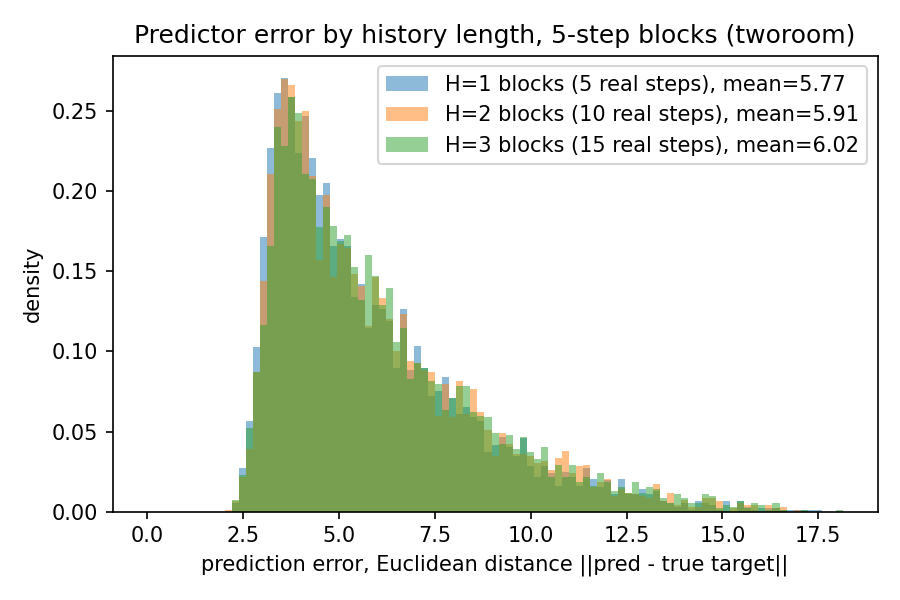
\includegraphics[width=0.75\linewidth]{figures/tworoom_predictor_error_by_history.png}
\caption{Predictor error (Euclidean distance between the prediction and the real target)
using the CORRECT 5-action-block convention, at $H{=}1,2,3$ blocks of history ($5,10,15$
real steps of context respectively), on 5000 real chains per length. Error is essentially
flat across $H$ --- means $5.77$, $5.91$, $6.02$ --- confirming (now on solid ground) that
extra history does not sharpen the one-block prediction for Two-Room, consistent with its
documented history length of $1$ and its genuinely memoryless dynamics (position and action
fully determine the next position).}
\label{fig:predictor-history}
\end{figure}

\begin{figure}[H]
\centering
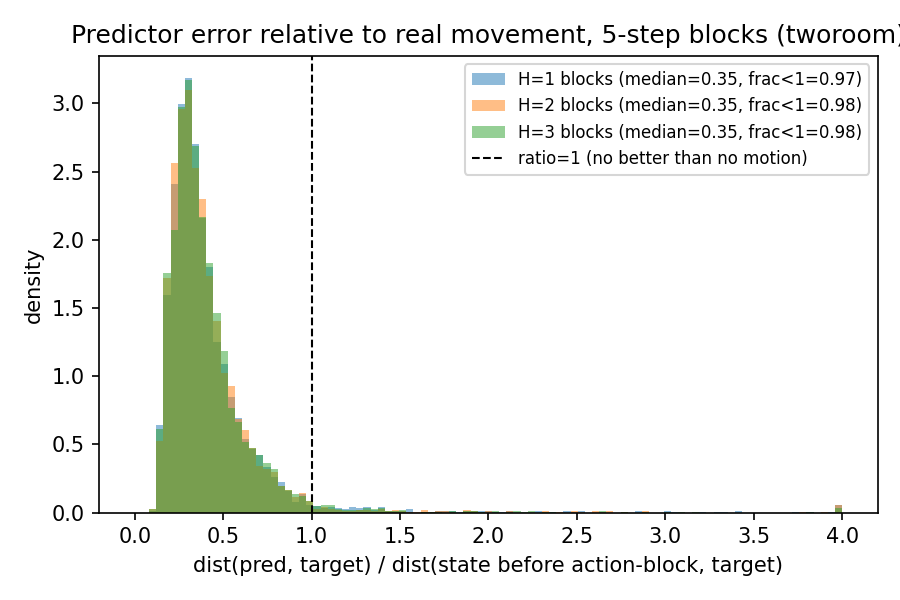
\includegraphics[width=0.75\linewidth]{figures/tworoom_predictor_ratio_by_history.png}
\caption{The same comparison, normalized: $\mathrm{dist}(\mathrm{pred},\mathrm{target}) /
\mathrm{dist}(\mathrm{state\ before\ the\ block},\mathrm{target})$. Median ratio
$\approx 0.35$ at every $H$, with $97$--$98\%$ of blocks showing \emph{some} improvement and
$\approx 78\%$ showing a strong one ($<0.5$) --- a real, substantial predictive signal, a
sharp contrast with the flawed single-action version this replaces (which showed no signal
at all under the wrong invocation).}
\label{fig:predictor-ratio}
\end{figure}

\begin{figure}[H]
\centering
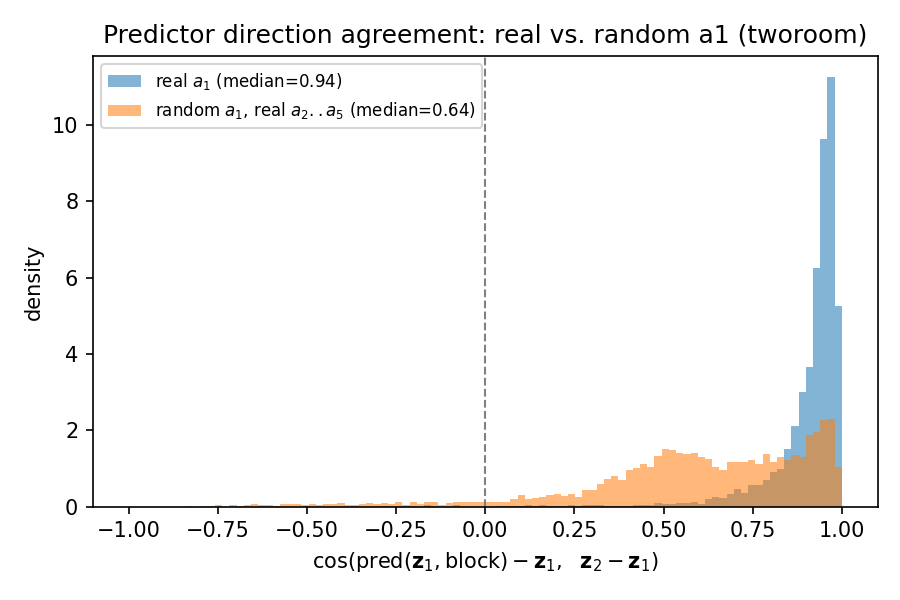
\includegraphics[width=0.75\linewidth]{figures/tworoom_predictor_direction_agreement.png}
\caption{Direction agreement on a real one-block ($H{=}1$, 5-real-step) transition, with a
control: $\cos(\mathrm{pred}(\zv_1,\mathrm{block}) - \zv_1,\ \zv_2 - \zv_1)$ using the real
$a_1$ (mean $0.905$, median $0.943$, $98.4\%$ above $0.5$) versus replacing $a_1$ with a
\emph{random} real action while keeping $a_2,\dots,a_5$ exactly as they really occurred
(mean $0.603$, median $0.641$, only $69.6\%$ above $0.5$). The real-$a_1$ numbers are even
better than the earlier (wrongly-invoked) figure this replaces. More importantly, the drop
under the random-$a_1$ control ($0.943\to0.641$) confirms the model genuinely weighs the
first action, not just the last four --- if it didn't, random and real $a_1$ would score
about the same. This is the control that makes \cref{fig:splice-verification}'s positive
result meaningful: the IDM's inferred action being indistinguishable from a real one is not
explainable by ``any $a_1$ would look fine here.''}
\label{fig:predictor-direction}
\end{figure}

\begin{figure}[H]
\centering
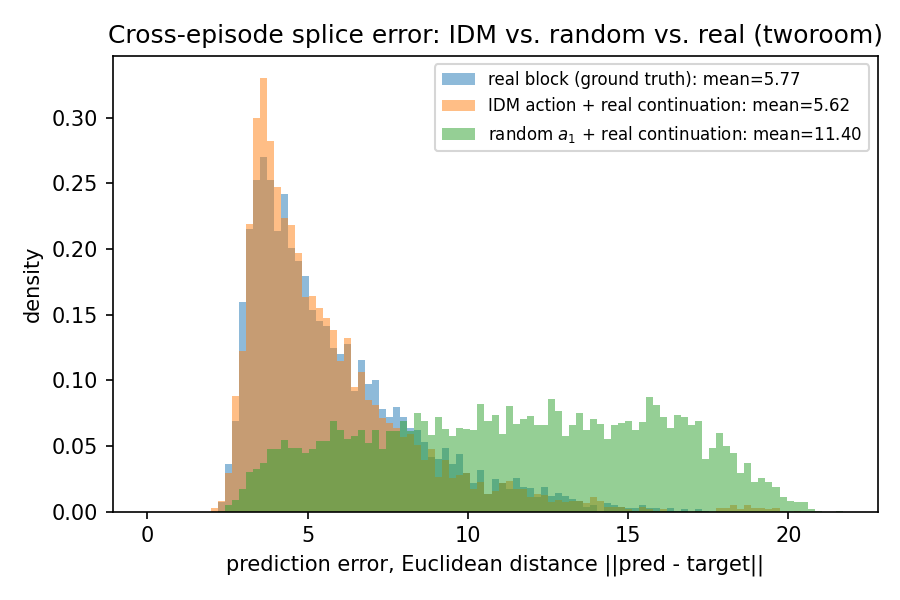
\includegraphics[width=0.75\linewidth]{figures/tworoom_splice_vs_ground_truth.png}
\caption{The real test this whole correction was for: does an IDM-inferred connecting
action, for a candidate cross-episode pair $(\zv_i,\zv_j)$ from the wide top-20 pool, work
as well as a genuine action once actually run through the predictor --- and does it do
\emph{better} than an uninformed guess? Three conditions, all predicting from $\zv_i$
against $\zv_{j+4}$ (where $j$'s own real rollout actually goes after its own next 4
actions): the hybrid block $(a,\ a_j,\ a_{j+1},\ a_{j+2},\ a_{j+3})$ with the IDM's inferred
$a$; the same block with $a$ replaced by a \emph{random} real action (the control); and the
reference (ground truth), \cref{fig:predictor-history}'s $H{=}1$ real block error. Result:
\textbf{IDM hybrid mean $5.62$, median $4.84$ --- indistinguishable from the real reference
(mean $5.77$, median $5.03$) --- while the random-$a_1$ control is mean $11.40$, median
$11.51$, roughly double both.} This is the decisive version of the earlier figure: the IDM's
inferred action is not merely ``fine because $j$'s own continuation carries the block
regardless of $a_1$'' (\cref{fig:predictor-direction} already suggested this, but this
figure confirms it directly in the actual cross-episode setting) --- a wrong first action
here is clearly and substantially worse, so the IDM's specific inference is doing real,
identifiable work.}
\label{fig:splice-verification}
\end{figure}

\textbf{Implication for \texttt{predictor-stitching.tex}'s E2 investigation.} Every
predictor call in that document's stages 1 and 3 (the absolute floor, direction agreement,
and relative-improvement criteria) used the same wrong single-action invocation this section
just corrected. Those results are not automatically wrong --- Two-Room's numbers above
barely changed under the fix, since its simple dynamics tolerate the malformed input
reasonably well --- but they were never validated under the correct convention either, and
should be re-run with \texttt{build\_block\_history\_chains}-style calls before being trusted
as a final verdict on E2's acceptance criterion.

\begin{figure}[H]
\centering
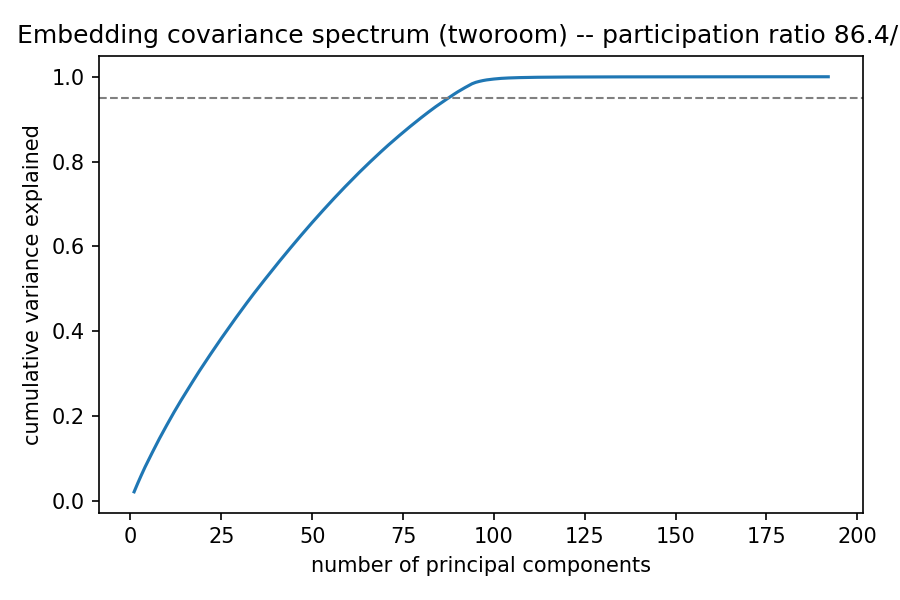
\includegraphics[width=0.75\linewidth]{figures/tworoom_pca_spectrum.png}
\caption{Cumulative variance explained by the embedding's principal components. Participation
ratio $86.4$ of $192$ ambient dimensions --- comparable to what \texttt{main.tex} measured on
Push-T ($84$ of $192$), despite Two-Room's calibration formula working and Push-T's failing
outright. Effective dimensionality alone does not predict which environment's calibration
holds; \texttt{main.tex}'s own diagnosis (its ``Diagnosing why the calibrated threshold
fails'' section) pins Push-T's failure on $\hat\rho$ itself, not on this.}
\label{fig:pca-spectrum}
\end{figure}

\begin{figure}[H]
\centering
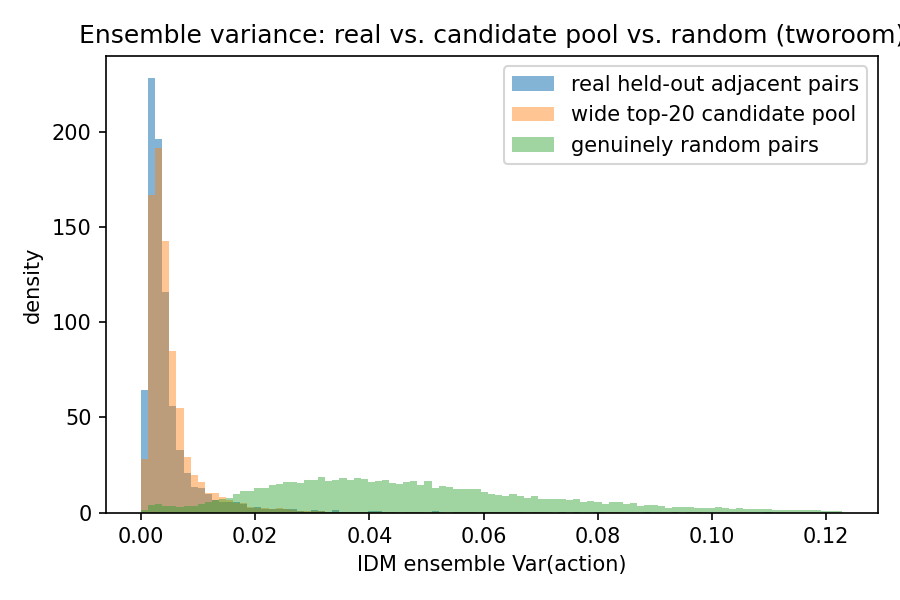
\includegraphics[width=0.75\linewidth]{figures/tworoom_idm_variance_comparison.png}
\caption{IDM ensemble variance on three populations: real held-out adjacent pairs (mean
$0.00505$, matching \texttt{predictor-stitching.tex}'s E1 result exactly), the wide top-20
candidate pool used in that document's E2 section (mean $0.00560$), and genuinely random,
unrelated state pairs (mean $0.0495$ --- an order of magnitude higher). Real transitions and
the candidate pool overlap almost completely, but both sit an order of magnitude below random
pairs. This changes how E2's finding should be read: variance is not an uninformative
signal in general --- it clearly separates ``a coherent single action connects these states''
from ``these are just two unrelated states'' --- it simply has little left to discriminate
\emph{within} the top-20 pool, because that pool is already overwhelmingly made of genuinely
connectable pairs, exactly as \texttt{predictor-stitching.tex}'s ground-truth environment
check (its E2 stage 2) independently found.}
\label{fig:idm-variance}
\end{figure}

\begin{figure}[H]
\centering
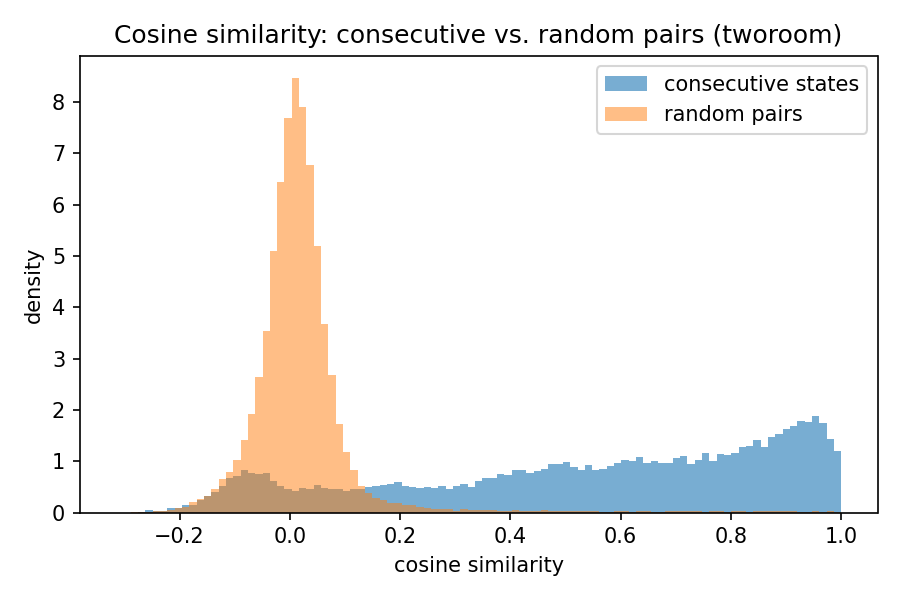
\includegraphics[width=0.75\linewidth]{figures/tworoom_cosine_similarity.png}
\caption{Cosine similarity between consecutive states (mean $0.540$) versus random pairs
(mean $0.021$, near the zero expected for near-orthogonal random vectors in $192$
dimensions). The adjacent-pair figure is close to $\hat\rho{=}0.584$ measured during
calibration --- consistent, since both summarize the same one-step correlation structure the
calibration formula is built on.}
\label{fig:cosine-similarity}
\end{figure}

\textbf{Follow-up already run:} \cref{fig:predictor-direction}'s direction-agreement result
was tried as a fix for \texttt{predictor-stitching.tex}'s E2 acceptance criterion (using the
IDM's inferred action on the candidate pool itself, gated on $\cos>0.5$) and made precision
worse, not better ($0.717\to0.609$) --- a distance-bucket breakdown there shows direction is
undefined for near-duplicate pairs (which dominate the pool) and non-target-specific at
larger gaps, so \cref{fig:predictor-direction}'s reliability on real transitions does not
transfer directly to this candidate pool's scale.

\textbf{Other diagnostics worth having if this line of work continues:} a version of
\cref{fig:predictor-direction} computed per raw-distance bucket rather than pooled, to see at
what scale (if any) direction agreement starts being genuinely target-specific rather than a
generic bias; per-tier versions of \cref{fig:adjacent-vs-random,fig:idm-variance} once a real
construction criterion is tested at scale (does the overlap in \cref{fig:idm-variance} change
with landmark count); the same figures repeated on Push-T, where
\cref{fig:random-vs-theoretical}'s close match and \cref{fig:pca-spectrum}'s participation
ratio are exactly the two things \texttt{main.tex} found behave differently; and a scatter of
IDM ensemble variance against true oracle distance (rather than the marginal histograms here)
to see directly whether any variance range corresponds to a reliable oracle-distance band,
not just whether the two populations' marginals overlap.

\end{document}
